\chapter{Numerical treatment of the fixed domain case}
\minitoc

\section{Introduction}

We will in this chapter be interested in the case of fixed domain Navier-Stokes with grid discretization.
This case is easier than the variable domain case and serves as a basis for more complicated cases.

We will treat the discretization of time and space separately.
We will first begin by time discretization.
The space discretization will only be used to evaluate derivatives.

We will in this chapter present two ways to solve the Navier-Stokes equations.
We will show that these two methods are equivalent if a Runge-Kutta method is used,
and that we are exactly divergence free.

In the next subsection we will present an overview of the two methods.

\subsection{Analytical expression for pressure}
\label{fixed:analytical}

We use the work of section \ref{analytical:fixe_eulerian} that Navier-Stokes equations are analytically equivalent to
\begin{equation}
  \partial_t \vect{v}(\vect{x} ,t)=(\eye-P)f(\vect{v}(\vect{x},t)).
\end{equation}

$\eye-P$ projects a non divergence free vector to obtain a divergence free vector.
The solution $\vect{v}$ is a divergence free vector as long that initial conditions are divergence free, because the integral of a divergence free vector is again a divergence free vector
\begin{align*}
 v(t)&=\int_{t_0}^{t}\partial_{\tilde{t}} \vect{v}(\vect{x} ,\tilde{t})=\int_{t_0}^{t} (\eye-P)f(\vect{v}(\vect{x},\tilde{t})) d\tilde{t}\\
 \vect{\nabla}\cdot v(t)&= \vect{\nabla}\cdot\int_{t_0}^{t} (\eye-P)f(\vect{v}(\vect{x},\tilde{t})) d\tilde{t}=\int_{t_0}^{t} \vect{\nabla}\cdot(\eye-P)f(\vect{v}(\vect{x},\tilde{t})) d\tilde{t}=\int_{t_0}^{t} 0 d\tilde{t}=0
\end{align*}


But a priori the numerical solution is not necessarily divergence free.

\subsection{Projection of speed}
\label{fixed:proj}

We can project every speed in a divergence free space
\begin{subequations}
\begin{align}
  \partial_t \vect{\tilde{v}}(\vect{x} ,t)&=f(\vect{v}(\vect{x},t)),\\
  \vect{v}(\vect{x},t)&=(\eye-P)\vect{\tilde{v}}.
\end{align}
\end{subequations}
$\vect{v}$ is certain to be always divergence free by construction.

\section{Time discretization and integration}
\label{fixed:timesec}
\subsection{Runge-Kutta method}

A Runge-Kutta method is a method to solve systems of ODEs (We drop the $\vect{x}$ dependence, but it is understood that this equation is for a vector formed in concatenating every speed)
\begin{equation}
\partial_t \vect{v}(t)=f(\vect{v}).
\end{equation}

The solution at time $n+1$ is given from the solution at time $n$ with $\Delta t$ the time step and $a$, $b$ parameters of the method,
\begin{subequations}
\begin{align}
	\vect{v}_{n+1}&=\vect{v}_{n}+\sum_{i=1}^{s}b_{i}\vect{k}_{i},\\
	\vect{k}_{i}&=\Delta t f(\vect{v}_{n}+\sum_{j=1}^{i-1}a_{ij}\vect{k}_{j}).
\end{align}
\end{subequations}

\subsection{Runge-Kutta based linear projection}
\label{fixed:sect:runge-kutta}
We now integrate equations given by methods (\ref{fixed:analytical}) and (\ref{fixed:proj}) with a Runge-Kutta method.

The numerical scheme for the exact divergence free speed is
\begin{subequations}
\begin{align}
\vect{\tilde{v}}_{n+1}&=(\eye-P)\vect{\tilde{v}}_{n}+\sum_{i=1}^{s}b_{i}\vect{\tilde{k}}_{i},\\
\vect{\tilde{k}}_{i}&=\Delta t f\left((\eye-P)\left(\vect{\tilde{v}}_{n}+\sum_{j=1}^{i-1}a_{ij}\vect{\tilde{k}}_{j}\right)\right).
\end{align}
\end{subequations}
We project at every input of the non linear $f$ function and at the final speed. Making by construction every speed divergence free.

Scheme for analytical expression for pressure:
\begin{subequations}
\begin{align}
	\vect{v}_{n+1}&=\vect{v}_{n}+\sum_{i=1}^{s}b_{i}\vect{k}_{i}\\
	k_{i}&=\Delta t f\left(\vect{v}_{n}+\sum_{j=1}^{i-1}a_{ij}\vect{k}_{j}\right)+\Delta t P\left(f\left(\vect{v}_{n}+\sum_{j=1}^{i-1}a_{ij}\vect{k}_{j}\right)\right)
\end{align}
\end{subequations}

The following theorem shows that the two schemes are the same.

\begin{theorem}
If $\vect{v}_{n}=\vect{\tilde{v}}_{n}$ and $\vect{v}_n$ is divergence free then $\vect{v}_{n+1}=\vect{\tilde{v}}_{n+1}$ 
\end{theorem}
\begin{proof}
We begin to prove the following lemma.
\begin{lemma}
\begin{equation}
  \vect{k}_{i}=\vect{\tilde{k}}_{i}+P(\vect{\tilde{k}}_{i})
\end{equation}
\end{lemma}
\begin{proof}
By recurrence on $i$.
We begin with $i=1$:
\begin{align}
  \vect{k}_{1}&=\Delta tf\left(\vect{v}_n\right)+\Delta tP\left(f\left(\vect{v}_n\right)\right)\\
\vect{\tilde{k}}_{1}&=\Delta tf\left(\vect{v}_n\right)\\
  \vect{k}_{1}&=\Delta t f\left(\vect{v}_n\right)+\Delta tP\left(f\left(\vect{v}_n\right)\right)=\vect{\tilde{k}}_1+P\left(\vect{\tilde{k}}_1\right)
\end{align}

Assuming true for smaller $i$:
\begin{align*}
  \vect{k}_{i}&=\Delta tf\left(\vect{v}_n+\sum_{j=1}^{n}a_{ij}k_{j}\right)+\Delta tP\left(f\left(\vect{v}_n+\sum_{j=1}^{i-1}a_{ij}\vect{k}_{j}\right)\right)\\
  \intertext{Using the recurrence relation we have:}
  &=\Delta tf\left(\vect{v}_n+\sum_{j=1}^{i-1}a_{ij}\left(\vect{\tilde{k}}_{j}+P\left(\vect{\tilde{k}}_{j}\right)\right)\right)+\Delta tP\left(f\left(\vect{v}_n+\sum_{j=1}^{i-1}a_{ij}\left(\vect{\tilde{k}}_{j}+P\left(\vect{\tilde{k}}_{j}\right)\right)\right)\right)\\
  \vect{\tilde{k}}_{i}&=\Delta tf\left(\vect{v}_n+\sum_{j=1}^{i-1}a_{ij}\vect{\tilde{k}}_{j}+P\left(\vect{v}_n+\sum_{j=1}^{i-1}a_{ij}\vect{\tilde{k}}_{j}\right)\right)\\
  \intertext{Using the linearity of $P$ and that $P\vect{v}_{n}=0$:}
  &=\Delta tf\left(\vect{v}_n+\sum_{j=1}^{i-1}a_{ij}\left(\vect{\tilde{k}}_{j}+P\left(\vect{\tilde{k}}_{j}\right)\right)\right)\\
  \vect{k}_{i}&=\vect{\tilde{k}}_{i}+P\left(\vect{\tilde{k}}_{i}\right)
\end{align*}
\end{proof}

We now write the expression for $\vect{v}_{n+1}$ and $\vect{\tilde{v}}_{n+1}$ using the lemma:
\begin{align*}
\vect{v}_{n+1}&=\vect{v}_{n}+\sum_{i=1}^{s}b_{i}\vect{k}_{i}\\
&=\vect{v}_{n}+\sum_{i=1}^{s}b_{i}\left(\vect{\tilde{k}}_{i}+P\left(\vect{\tilde{k}}_{i}\right)\right)\\
\vect{\tilde{v}}_{n+1}&=\vect{\tilde{v}}_{n}+\sum_{i=1}^{s}b_{i}\vect{\tilde{k}}_{i}+P\left(\vect{\tilde{v}}_{n}+\sum_{i=1}^{s}b_{i}\vect{\tilde{k}}_{i}\right)\\
\intertext{Using the linearity of $P$ and that $P\vect{\tilde{v}}_{n}=0$}
&=\vect{\tilde{v}}_{n}+\sum_{i=1}^{s}b_{i}\left(\vect{\tilde{k}}_{i}+P\left(\vect{\tilde{k}}_{i}\right)\right)\\
\intertext{Using that $\vect{v}_{n}=\tilde{\vect{v}}_{n}$}
\vect{v}_{n+1}&=\vect{\tilde{v}}_{n+1}
\end{align*}

\end{proof}

\begin{theorem}
For the implicit Runge-Kutta case, where the sum to $i-1$ goes now to $s$.
If $\vect{v}_{n}=\vect{\tilde{v}}_{n}$ and $\vect{v}_n$ is divergence free then $\vect{v}_{n+1}=\vect{\tilde{v}}_{n+1}$ 
\end{theorem}
\begin{proof}
We begin to prove the following lemma.
\begin{lemma}
After relabeling noting $\vect{k}_{i}^{j}$ the $j$-th solution of $\vect{k}_{i}$.
We have for every $j$.
\begin{equation}
  \vect{k}_{i}^{j}=\vect{\tilde{k}}_{i}^{j}+P(\vect{\tilde{k}}_{i}^{j})
\end{equation}
This doesn't say that we have existence and unicity of the solution only that if we have a set of solution for $\vect{k}$ we have a bijection
to solutions of $\vect{\tilde{k}}$
\end{lemma}
\begin{proof}
Because the sum goes to $s$ and not $i-1$ we cannot use recurrence.
We now will use vector notation for $k$.

We construct $k$ and $\tilde{k}$ vector with the vector $\vect{k}_{i}$ and $\vect{\tilde{k}}_{i}$
\begin{align}
k&=\begin{pmatrix}
    \vect{k}_{1}\\
    \vdots\\
    \vect{k}_{s}\\
  \end{pmatrix}\\
\tilde{k}&=\begin{pmatrix}
    \vect{\tilde{k}}_{1}\\
    \vdots\\
    \vect{\tilde{k}}_{s}\\
  \end{pmatrix}
\end{align}

We form $\hat{P}$ and $\hat{f}$ from a Kronecker product:
\begin{align}
\hat{P}&=\eye_{s}\kron P=\begin{pmatrix}P	&\ldots	&0\\
			\vdots &\ddots 	&\vdots\\
			0	&\ldots		&P\\
	\end{pmatrix}\\
\hat{f}&=\eye_{s}\kron f=\begin{pmatrix}f	&\ldots	&0\\
			\vdots &\ddots 	&\vdots\\
			0	&\ldots	&f\\
	\end{pmatrix}
\end{align}
Where for $\hat{f}$ we have used a notation where:
\begin{equation}
 \hat{f}\left(k\right)=\begin{pmatrix}f(\vect{k}_1)\\
			\vdots\\
			f(\vect{k}_n)\\
	\end{pmatrix}
\end{equation}


We now define $\hat{v}_n$:
\begin{equation}
\hat{v}_{n}=\begin{pmatrix}
	      \vect{v}_{n}\\
	      \vdots\\
	      \vect{v}_{n}
	      \end{pmatrix}
\end{equation}

We now define $\hat{A}$ with the following Kronecker product:
\begin{equation}
\hat{A}=\begin{pmatrix}
    a_{11}	&\ldots	&a_{1s}\\
    \vdots	&\ddots	&\vdots\\
    a_{s1}	&\ldots	&a_{ss}\\
  \end{pmatrix} \kron \eye=A \kron \eye
\end{equation}

$\hat{A}$ and $\hat{P}$ are commutative, because of the mixed-product property.
\begin{align}
\hat{A}\hat{P}&=\left(A\kron \eye \right)
  \left(\eye_{s}\kron P\right)=
	A\kron P\\
    %
    \hat{P}\hat{A}&=
  \left(\eye_{s}\kron P\right)
	\left(A \kron \eye \right)=
	A\kron P
\end{align}

The two expressions can now be written:
\begin{align}
k&=(1+\hat{P})\Delta t\hat{f}(\hat{v}_{n}+\hat{A}k)\\
\tilde{k}&=\Delta t \hat{f}((1+\hat{P})(\hat{v}_{n}+\hat{A}k))
\end{align}

We begin to define 2 functions:
\begin{align}
k&=g(k)\\
\tilde{k}&=\tilde{g}(\tilde{k})\\
g(x)&=(1+\hat{P})\Delta t \hat{f}(\hat{v}_{n}+\hat{A}x)\\
\tilde{g}(x)&=\Delta t \hat{f}((1+\hat{P})(\hat{v}_{n}+\hat{A}x))
\end{align}

$k$ and $\tilde{k}$ are fixed points of functions $g$ and $\tilde{g}$.

We now calculate:
\begin{align}
(1+\hat{P})\tilde{g}(x)&=(1+\hat{P})\Delta t \hat{f}((1+\hat{P})(\hat{v}_{n}+\hat{A}x))\\
\intertext{Using:}
\hat{P}\hat{v}_{n}=0
\intertext{Using that $\hat{A}$ and $\hat{P}$ commute}
(1+\hat{P})\tilde{g}(x)&=(1+\hat{P})\Delta t \hat{f}(\hat{v}_{n}+\hat{A} (1+\hat{P})x)\\
&=g((1+\hat{P})x)
\end{align}

We now substitute $x$ with $\tilde{k}$
\begin{align}
(1+\hat{P})\tilde{g}(\tilde{k})&=g((1+\hat{P})\tilde{k})
\intertext{by definition $\tilde{k}$ is a fixed point of $\tilde{g}$}
(1+\hat{P})\tilde{k}&=g((1+\hat{P})\tilde{k})
\end{align}
$(1+\hat{P})\tilde{k}$ is a fixed point of $g$.
But fixed point of $g$ is $k$.

With relabeling of solution if needed, this directly gives the result with $\vect{k}^{j}$ the $j$-th solution:
\begin{equation}
\vect{k}^{j}=(1+\hat{P})\vect{\tilde{k}}^{j}
\end{equation}
This is exactly the vector version of what we wanted to prove.
\end{proof}

The rest is exactly the same than in the first case.
To not overload the proof with notation, we drop the $j$ label to indicate which solution we take.

We now write the expression for $\vect{v}_{n+1}$ and $\vect{\tilde{v}}_{n+1}$ using the lemma.
\begin{align*}
\vect{v}_{n+1}&=\vect{v}_{n}+\sum_{i=1}^{s}b_{i}\vect{k}_{i}\\
&=\vect{v}_{n}+\sum_{i=1}^{s}b_{i}\left(\vect{\tilde{k}}_{i}+P\left(\vect{\tilde{k}}_{i}\right)\right)\\
\vect{\tilde{v}}_{n+1}&=\vect{\tilde{v}}_{n}+\sum_{i=1}^{s}b_{i}\vect{\tilde{k}}_{i}+P\left(\vect{\tilde{v}}_{n}+\sum_{i=1}^{s}b_{i}\vect{\tilde{k}}_{i}\right)\\
&=\vect{\tilde{v}}_{n}+\sum_{i=1}^{s}b_{i}\left(\vect{\tilde{k}}_{i}+P\left(\vect{\tilde{k}}_{i}\right)\right)\\
\intertext{Using that $\vect{v}_{n}=\tilde{\vect{v}_{n}}$}
\vect{v}_{n+1}&=\vect{\tilde{v}}_{n+1}
\end{align*}

\end{proof}

\begin{corollary}
Solving Navier-Stokes equation with the analytical good choice of pressure is exactly divergence free at every approximation of speed.
\end{corollary}
\begin{proof}
  The expression of $\vect{v}$ is the solution of the Navier-Stokes equation with the good choice of pressure.
  $\vect{\tilde{v}}$ is the solution of Runge-Kutta equation without pressure which is projected at every speed estimation.
  $\vect{v}$ and $\vect{\tilde{v}}$ are the same by the theorem.
\end{proof}

\begin{corollary}
  Using the expression for $\vect{v}$ or $\vect{\tilde{v}}$ we are $k$ order precise in time. Where $k$ is the order of the Runge-Kutta method.
\end{corollary}
\begin{proof}
  $\vect{v}$ and $\vect{\tilde{v}}$ are the same.
  $\vect{v}$ consists only of a Runge-Kutta method with a good chosen function.
  So the order in time of $\vect{v}$ and $\vect{\tilde{v}}$ is the same that the method order.
\end{proof}


\subsection{Runge-Kutta based affine projection}
\label{fixed:sect:runge-kutta:affine}
We will repeat the work in section \ref{fixed:sect:runge-kutta} but where the projection is an affine operator.
We use the notation of \ref{introduction:projectiondef}.

Scheme for projection at every evaluation of speed:
\begin{subequations}
\begin{align}
\vect{\tilde{v}}_{n+1}&=\vect{\tilde{v}}_{n}+\sum_{i=1}^{s}b_{i}\vect{\tilde{k}}_{i}+P\left(\vect{\tilde{v}}_{n}+\sum_{i=1}^{s}b_{i}\vect{\tilde{k}}_{i},\vect{\tilde{T}}_0\right)\\
\vect{\tilde{k}}_{i}&=\Delta t f\left(\vect{\tilde{v}}_{n}+\sum_{j=1}^{i-1}a_{ij}\vect{\tilde{k}}_{j}+P\left(\vect{\tilde{v}}_{n}+\sum_{j=1}^{i-1}a_{ij}\vect{\tilde{k}}_{j},\vect{\tilde{T}}_i\right)\right)
\end{align}
\end{subequations}
We project at every estimation of speed. Making by construction every speed divergence free.

Scheme for analytical expression for pressure:
\begin{subequations}
\begin{align}
	\vect{v}_{n+1}&=\vect{v}_{n}+\sum_{i=1}^{s}b_{i}\vect{k}_{i}\\
	\vect{k}_{i}&=\Delta t f\left(\vect{v}_{n}+\sum_{j=1}^{i-1}a_{ij}\vect{k}_{j}\right)+\Delta t P\left(f\left(\vect{v}_{n}+\sum_{j=1}^{i-1}a_{ij}\vect{k}_{j}\right),\vect{T}_{i}\right)
\end{align}
\end{subequations}

The following theorem shows that the two schemes are the same and give the relation between $T$ and $\tilde{T}$.

\begin{theorem}
If $\vect{v}_{n}=\vect{\tilde{v}}_{n}$ and $\vect{v}_n$ are divergence free then $\vect{v}_{n+1}=\vect{\tilde{v}}_{n+1}$.
With the relation for the translation:
\begin{align}
\intertext{For $0< i\leq s$}
  \vect{\tilde{T}}_i&=\sum_{j=1}^{i-1}a_{ij}\Delta t \vect{T}_{j}\\
  \vect{\tilde{T}}_0&=\sum_{i=1}^{s}b_{i}\Delta t \vect{T}_{i}
\end{align}

\end{theorem}
\begin{proof}
We begin to prove the following lemma.
\begin{lemma}
\begin{equation}
  \vect{k}_{i}=\vect{\tilde{k}}_{i}+P(\vect{\tilde{k}}_{i},\Delta t \vect{T}_{i})
\end{equation}
\end{lemma}
\begin{proof}
By recurrence on $i$.
We begin with $i=1$:
\begin{align}
  \vect{k}_{1}&=\Delta tf\left(\vect{v}_n\right)+\Delta tP\left(f\left(\vect{v}_n\right),\vect{T}_{1}\right)\\
\vect{\tilde{k}}_{1}&=\Delta tf\left(\vect{\vect{v}}_n\right)\\
  \vect{k}_{1}&=\Delta t f\left(\vect{v}_n\right)+\Delta tP\left(f\left(\vect{v}_n\right),\vect{T}_{1}\right)=\vect{\tilde{k}}_1+P\left(\vect{\tilde{k}}_1,\Delta t \vect{T}_{1}\right)
\end{align}

Assuming true for smaller $i$:
\begin{align*}
  \vect{k}_{i}&=\Delta tf\left(\vect{v}_n+\sum_{j=1}^{n}a_{ij}\vect{k}_{j}\right)+\Delta tP\left(f\left(\vect{v}_n+\sum_{j=1}^{i-1}a_{ij}\vect{k}_{j}\right),\vect{T}_{i}\right)\\
  &=\Delta tf\left(\vect{v}_n+\sum_{j=1}^{i-1}a_{ij}\left(\vect{\tilde{k}}_{j}+P\left(\vect{\tilde{k}}_{j},\Delta t \vect{T}_{j}\right)\right)\right)+\Delta tP\left(f\left(\vect{v}_n+\sum_{j=1}^{i-1}a_{ij}\left(\vect{\tilde{k}}_{j}+P\left(\vect{\tilde{k}}_{j},\Delta t \vect{T}_{j}\right)\right)\right),\vect{T}_{i}\right)\\
  \vect{\tilde{k}}_{i}&=\Delta tf\left(\vect{v}_n+\sum_{j=1}^{i-1}a_{ij}\vect{\tilde{k}}_{j}+P\left(\vect{v}_n+\sum_{j=1}^{i-1}a_{ij}\vect{\tilde{k}}_{j},\vect{\vect{\tilde{T}}}_{i}\right)\right)\\
  \intertext{Using the linearity of $P$ and $P\vect{v}_n=0$ and defining $\vect{\hat{T}}_{j}^i$}
  &=\Delta tf\left(\vect{v}_n+\sum_{j=1}^{i-1}a_{ij}\left(\vect{\tilde{k}}_{j}+P\left(\vect{\tilde{k}}_{j},\vect{\hat{T}}_{j}^{i}\right)\right)\right)\\
  \vect{\tilde{T}}_i&=\sum_{j}^{i-1}a_{ij}\vect{\hat{T}}_{j}^{i}\\
  \vect{\hat{T}}^{i}_{j}&=\Delta t \vect{T}_{j}\\
  \vect{k}_{i}&=\vect{\tilde{k}}_{i}+P\left(\vect{\tilde{k}}_{i},\Delta t\vect{T}_j\right)
\end{align*}
This prove the relation and give the relation between the two.
\begin{equation}
  \vect{\tilde{T}}_i=\sum_{j}^{i-1}a_{ij}\Delta t \vect{T}_{j}
\end{equation}
\end{proof}

We now write the expression for $\vect{v}_{n+1}$ and $\vect{\tilde{v}}_{n+1}$ using the lemma.
\begin{align*}
\vect{v}_{n+1}&=\vect{v}_{n}+\sum_{i=1}^{s}b_{i}\vect{k}_{i}\\
&=\vect{v}_{n}+\sum_{i=1}^{s}b_{i}\left(\vect{\tilde{k}}_{i}+P\left(\vect{\tilde{k}}_{i},\Delta t\vect{T}_{i}\right)\right)\\
\vect{\tilde{v}}_{n+1}&=\vect{\tilde{v}}_{n}+\sum_{i=1}^{s}b_{i}\vect{\tilde{k}}_{i}+P\left(\vect{\tilde{v}}_{n}+\sum_{i=1}^{s}b_{i}\vect{\tilde{k}}_{i},\vect{\tilde{T}}_{0}\right)\\
&=\vect{\tilde{v}}_{n}+\sum_{i=1}^{s}b_{i}\left(\vect{\tilde{k}}_{i}+P\left(\vect{\tilde{k}}_{i},\vect{\hat{T}}_{i}^{0}\right)\right)\\
\vect{\tilde{T}}_{0}&=\sum_{i=1}^{s}b_{i}\vect{\hat{T}}_{i}^{0}\\
\vect{\tilde{T}}_{0}&=\sum_{i=1}^{s}b_{i}\Delta t \vect{T}_{i}\\
\intertext{Using that $\vect{v}_{n}=\tilde{\vect{v}}_{n}$}
\vect{v}_{n+1}&=\vect{\tilde{v}}_{n+1}
\end{align*}

\end{proof}

\begin{theorem}
For the implicit Runge-Kutta case, where the sum on $i-1$ goes now to $s$.
If $\vect{v}_{n}=\vect{\tilde{v}}_{n}$ and $\vect{v}_n$ are divergence free then $\vect{v}_{n+1}=\vect{\tilde{v}}_{n+1}$.
And the translation is given by:
\begin{align}
  \vect{\tilde{T}}_{i}&=\Delta t\sum_{j}a_{ij}\vect{T}_{j}\\
  \vect{\tilde{T}}_{0}&=\Delta t\sum_{j}b_{j}\vect{T}_{j}
\end{align}

\end{theorem}
\begin{proof}
We begin to prove the following lemma.
\begin{lemma}
After relabeling $j$ noting $\vect{k}_{i}^{j}$ the $j$ solution of $\vect{k}_{i}$.
We have for every $j$.
\begin{equation}
  \vect{k}_{i}^{j}=\vect{\tilde{k}}_{i}^{j}+P(\vect{\tilde{k}}_{i}^{j},\Delta t \vect{T}_{i})
\end{equation}
This doesn't say that we have existence and unicity of the solution only that if we have a set of solution for $k$ we have a bijection
to solution of $\tilde{k}$
\end{lemma}
\begin{proof}
Because the sum goes to $s$ and not $i-1$ we cannot use recurrence.
We now will use vector notation for $k$.

We construct $k$ and $\tilde{k}$ vectors with the vector $\vect{k}_{i}$ and $\vect{\tilde{k}}_{i}$
\begin{align}
k&=\begin{pmatrix}
    \vect{k}_{1}\\
    \vdots\\
    \vect{k}_{s}\\
  \end{pmatrix}\\
\tilde{k}&=\begin{pmatrix}
    \vect{\tilde{k}}_{1}\\
    \vdots\\
    \vect{\tilde{k}}_{s}\\
  \end{pmatrix}
\end{align}

We form $\hat{L}$ the linear part of the projection from $L$ the linear part from the projection $P$.
\begin{align}
\hat{L}&=\eye_{s}\kron L=\begin{pmatrix}L	&\ldots	&0\\
			\vdots &\ddots 	&\vdots\\
			0	&\ldots	&L\\
	\end{pmatrix}
\end{align}
We have the following property:
\begin{equation}
\hat{L}\hat{v}_{n}=0
\end{equation}
This is true because $\hat{v}_{n}$ is divergence free.
$\hat{L}$ is the linear part and consist to make the projection with 0 boundary conditions.

$\tau_{i}$ the translation vector from $\vect{T}_i$ the translation part of $P$.
$\tau$ is the sum of all individual translation.
\begin{align}
	\tau_i&=\begin{pmatrix}
			\vect{0}\\
			\vdots\\
			\vect{T}_{i}\\
			\vdots\\
			\vect{0}\\
	\end{pmatrix}
	\\
	\tau&=\sum_{i}\tau_{i}=\begin{pmatrix}
			\vect{T}_{1}\\
			\vdots\\
			\vect{T}_{s}\\
	\end{pmatrix}
\end{align}

Same for $\tilde{\tau}_{i}$ with $\vect{T}_{i}$ changed with $\vect{\tilde{T}}_i$

We now form the function $\hat{f}$ from $f$ with:
\begin{align}
\hat{f}&=\eye_{s}\kron f=\begin{pmatrix}f	&\ldots	&0\\
			\vdots &\ddots 	&\vdots\\
			0	&\ldots	&f\\
	\end{pmatrix}
\end{align}

We now define $\hat{v}_n$:
\begin{equation}
\hat{v}_{n}=\begin{pmatrix}
	      \vect{v}_{n}\\
	      \vdots\\
	      \vect{v}_{n}
	      \end{pmatrix}
\end{equation}

We now define $\hat{A}$ with the following Kronecker product:
\begin{equation}
\hat{A}=\begin{pmatrix}
    a_{11}	&\ldots	&a_{1s}\\
    \vdots	&\ddots	&\vdots\\
    a_{s1}	&\ldots	&a_{ss}\\
  \end{pmatrix} \kron \eye=A \kron \eye
\end{equation}

$\hat{A}$ and $\hat{L}$ are commutative, because of the mixed-product property.
\begin{align}
\hat{A}\hat{L}&=\left(A\kron \eye \right)
  \left(\eye_{s}\kron L\right)=
	A\kron L\\
    %
    \hat{L}\hat{A}&=
  \left(\eye_{s}\kron L\right)
	\left(A \kron \eye \right)=
	A\kron L
\end{align}

\begin{align}
k&=(1+\hat{L})\Delta t\hat{f}(\hat{v}_{n}+\hat{A}k)+\Delta t\tau\\
\tilde{k}&=\Delta t \hat{f}((1+\hat{L})(\hat{v}_{n}+\hat{A}k)+\tilde{\tau})
\end{align}

We begin to define 2 functions:
\begin{align}
k&=g(k)\\
\tilde{k}&=\tilde{g}(\tilde{k})\\
g(x)&=(1+\hat{L})\Delta t \hat{f}(\hat{v}_{n}+\hat{A}x)+\Delta t\tau\\
\tilde{g}(x)&=\Delta t \hat{f}((1+\hat{L})(\hat{v}_{n}+\hat{A}x)+\tilde{\tau})
\end{align}

$k$ and $\tilde{k}$ are fixed points of function $g$ and $\tilde{g}$.

We now calculate using that $L$ is linear and $L\hat{v}=0$:
\begin{align}
(1+\hat{L})\tilde{g}(x)&=(1+\hat{L})\Delta t \hat{f}((1+\hat{L})(\hat{v}_{n}+\hat{A}x)+\tilde{\tau})=(1+\hat{L})\Delta t \hat{f}(\hat{v}_{n}+\hat{A} (1+\hat{L})x+\tilde{\tau})\\
&=(1+\hat{L})\Delta t \hat{f}(\hat{v}_{n}+\hat{A} ((1+\hat{L})x+\hat{A}^{-1}\tilde{\tau}))\\
\intertext{By definition of $g$ we have:}
&=g((1+\hat{L})x+\hat{A}^{-1}\tilde{\tau})-\Delta t \tau
\end{align}

We now substitute $\tilde{k}$ in $x$
\begin{align}
(1+\hat{L})\tilde{g}(\tilde{k})&=g((1+\hat{L})\tilde{k}+\hat{A}^{-1}\tilde{\tau})-\Delta t \tau\\
\intertext{$\tilde{k}$ is a fixed point of $\tilde{g}$}
(1+\hat{L})\tilde{k}&=g((1+\hat{L})\tilde{k}+\hat{A}^{-1}\tilde{\tau})-\Delta t \tau\\
(1+\hat{L})\tilde{k}+\Delta t \tau&=g((1+\hat{L})\tilde{k}+\hat{A}^{-1}\tilde{\tau})\\
\intertext{If}
\tilde{\tau}=\Delta t \hat{A}\tau
\intertext{Then}
(1+\hat{L})\tilde{k}+\Delta t \tau&=g((1+\hat{L})\tilde{k}+\Delta t \tau)
\end{align}
$(1+\hat{L})\tilde{k}+\Delta t \tau$ is a fixed point of $g$.
But fixed point of $g$ is $k$.

After relabeling of solution, this directly gives the result with $k^{j}$ the $j$-th solution:
\begin{equation}
k^{j}=(1+\hat{L})\tilde{k}^{j}+\Delta t \tau
\end{equation}
This is exactly the vector version of what we wanted to prove.
\end{proof}

The rest is exactly the same than in the first case.
To not overload the proof with notation, we drop the $j$ label to indicate which solution we take.

We now write the expression for $\vect{v}_{n+1}$ and $\vect{\tilde{v}}_{n+1}$ using the lemma.
\begin{align*}
\vect{v}_{n+1}&=\vect{v}_{n}+\sum_{i=1}^{s}b_{i}\vect{k}_{i}\\
&=\vect{v}_{n}+\sum_{i=1}^{s}b_{i}\left(\left(\eye+L\right)\vect{\tilde{k}}_i+\Delta t \vect{T}_{i}\right)\\
\vect{\tilde{v}}_{n+1}&=\vect{\tilde{v}}_{n}+\sum_{i=1}^{s}b_{i}\vect{\tilde{k}}_{i}+L\left(\vect{\tilde{v}}_{n}+\sum_{i=1}^{s}b_{i}\vect{\tilde{k}}_{i}\right)+\vect{\tilde{T}}_0\\
&=\vect{\tilde{v}}_{n}+\sum_{i=1}^{s}b_{i}\left(\eye+L\right)\vect{\tilde{k}}_{i}+\vect{\tilde{T}}_0\\
\vect{\tilde{T}}_0&=\Delta t\sum_{i=1}^{s}b_{i}\vect{T}_{i}\\
\intertext{Using that $\vect{v}_{n}=\tilde{\vect{v}}_{n}$}
\vect{v}_{n+1}&=\vect{\tilde{v}}_{n+1}
\end{align*}

\end{proof}

\section{Spatial discretization}

\subsection{Non-staggered grid}

On a non-staggered grid we put the variable like figure \ref{fixed:unstaggered}.
\begin{figure}
\directlua{dofile('fixed/unstaggered.lua')}
\caption{Position of variable for Non-Staggered grid}
\label{fixed:unstaggered}
\end{figure}
The problem with non-staggered  grid, is that obvious center difference discretization lead to wrong divergence free vector.

We define the derivative of a scalar by:
\begin{equation}
  \partial_x a_i=\frac{a_{i+1}-a{i-1}}{\Delta x}
\end{equation}
The divergence discretization is then given by (notation for 2d, but for 3d it's the same):
\begin{equation}
  \vect{\nabla} \cdot \vect{v}_{i,j}=\frac{{v_{x}}_{i+1,j}-{v_{x}}_{i-1,j}}{\Delta x}+\frac{{v_{y}}_{i+1,j}-{v_{y}}_{i-1,j}}{\Delta y}
\end{equation}
The problem can be seen in figure \ref{fixed:unstaggered_div} is that the divergence at red point only use value at blue point and not the point at center (red point).
This allows to have non-physical solutions that are divergence free.

\begin{figure}
\directlua{dofile('fixed/unstaggered_div.lua')}
\caption{Values used to calculate the divergence at red point are in blue}
\label{fixed:unstaggered_div}
\end{figure}

In figure \ref{fixed:unstaggered_div2} we have a solution that is numerically divergence free.
But this solution is not continuous and we expect that is not divergence free.

\begin{figure}
\directlua{dofile('fixed/unstaggered_div2.lua')}
\caption{Speed that are numerically divergence free but shouldn't}
\label{fixed:unstaggered_div2}
\end{figure}

The problem with this kind of solution, is that it's very stable.
The projection operator $P$ will be 0, and doesn't correct this kind of speed. We cannot correct it in general for every choice of $f$.
Note that all the work done in section \ref{fixed:timesec} is true. In particular the theorem will be true and will correctly projects
in a divergence free space. It's only that our divergence free space contains solutions that are not wanted.

We can recall one of the formulations of the so called Murphy's law, ``If anything can go wrong, it will.''

We can correct this problem with using a forward or backward expression. But this kind of expression is only first order accurate.
Another solution is to use another grid.

\FloatBarrier
\subsection{Staggered grid}

On a staggered grid we put the variable in the position shown if figure \ref{fixed:staggered}.
\begin{figure}
\directlua{dofile('fixed/staggered.lua')}
\caption{Position of variable on a staggered grid}
\label{fixed:staggered}
\end{figure}

This can seem to be strange to have different component of speed at different places. But it make discretization more easy.
To label variable, we label by cell and then took the lower left component (cf. figure \ref{fixed:staggered_label}).
\begin{figure}
\directlua{dofile('fixed/staggered_label.lua')}
\caption{Labeling on staggered grid}
\label{fixed:staggered_label}
\end{figure}

We now define the divergence and the gradient:
\begin{align}
  \vect{\nabla}p_{ij}&=\begin{pmatrix}
    \frac{p_{i,j}-p_{i-1,j}}{\Delta x}\\
    \frac{p_{i,j}-p_{i,j-1}}{\Delta y}\\
                      \end{pmatrix}\\
  \vect{\nabla}\cdot \vect{v}_{i,j}&=\frac{{v_{x}}_{i+1,j}-{v_{x}}_{i,j}}{\Delta x}+\frac{{v_{y}}_{i,j+1}-{v_{y}}_{i,j}}{\Delta y}
\end{align}
This two expressions are geometrically very clear.

In figure \ref{fixed:staggered_gradient}, the gradient at red speed component uses components at blue point.
Contrary at case with center difference we cannot create a none constant vector with 0 gradient.
\begin{figure}
\directlua{dofile('fixed/staggered_gradient.lua')}
\caption{Points used to calculate the red gradient component are in blue}
\label{fixed:staggered_gradient}
\end{figure}

The divergence is given by the sum of inflow around a cell.
In figure \ref{fixed:staggered_divergence}, the divergence at red point uses components at blue point.
\begin{figure}
\directlua{dofile('fixed/staggered_divergence.lua')}
\caption{Points used to calculate red divergence are in blue}
\label{fixed:staggered_divergence}
\end{figure}

We cannot have the same situation than without staggered grid, where a nonphysical vector is divergence free.

\subsubsection{Discretization}

We now look at different possible schemes for staggered grid discretization.

\paragraph{Gradient}
\label{fixed:gradient}

The gradient is discretized with center difference.
\begin{equation}
  \vect{\nabla}p_{i,j}=\begin{pmatrix}
                       	\frac{p_{i-1,j}-p_{i,j}}{\Delta x}\\
                       	\frac{p_{i,j-1}-p_{i,j}}{\Delta y}\\
                       \end{pmatrix}
\end{equation}
Center difference is second order accurate to the contrary of forward or backward difference.

\paragraph{Divergence}
\label{fixed:divergence}

The divergence is discretized with center difference.
\begin{equation}
	\vect{\nabla}\cdot \vect{v}_{i,j}=\frac{{v_{x}}_{i,j}-{v_{x}}_{i-1,j}}{\Delta x}+\frac{{v_{y}}_{i,j}-{v_{y}}_{i,j-1}}{\Delta y}
\end{equation}
Because of center difference its second order accurate.

\paragraph{Laplacian}
\label{fixed:Laplacian}

The discretization of the Laplacian is the combination of the application of the gradient and divergence.
\begin{equation}
  \Delta p_{i,j}=\frac{p_{i+1,j}-2p_{i,j}+p_{i-1,j}}{(\Delta x)^2}+\frac{p_{i,j+1}-2p_{i,j}+p_{i,j-1}}{(\Delta y)^2}
\end{equation}
This formula is of order 2.
We prove it for the one dimensional case:
\begin{align*}
  f(x+\Delta x)-2f(x)+f(x-\Delta x)&=\\
  \intertext{We make a Taylor expansion around $x$}
  &=f(x)+\Delta x f'(x) +(\Delta x)^2 \frac{f''(x)}{2}+(\Delta x)^3 \frac{f'''(x)}{6}+O((\Delta x)^4)-2f(x)\\
  &\qquad+f(x)-\Delta x f'(x) +(\Delta x)^2 \frac{f''(x)}{2}-(\Delta x)^3 \frac{f'''(x)}{6}\\
  &=(\Delta x)^2f''(x) +O((\Delta x)^4)\\
  f''(x)&=\frac{f(x+\Delta x)-2f(x)+f(x-\Delta x)}{(\Delta x)^2}+O((\Delta x)^2)
\end{align*}

\paragraph{Vector laplacian}
\label{fixed:vect:laplacian}
For vector Laplacian we use the same scheme as in section \ref{fixed:Laplacian} but for every component of speed.
Staggered grid doesn't pose problem because we don't have mixed terms with derivative and non derivative.

\paragraph{Convection}

Convection term is the more difficult term to treat, because it's non linear and uses mixed terms.
We need to consider two type of terms. Let $i\neq j$ and $\vect{k}$ be an integer vector of the position on the grid
and $\vect{e}_i$ the $i$-th unit vector.
We first consider as $i$-th component:
\begin{equation}
\left(v^{i}\partial_{i}v^{i}\right)^{i}_{\vect{k}}
\end{equation}
We can discretize this in two manners:

\subparagraph{Central difference}
\begin{equation}
{v^{i}}_{\vect{k}}\frac{{v^{i}}_{\vect{k}+\vect{e}_i}-{v^{i}}_{\vect{k}-\vect{e}_i}}{2\Delta x_{i}}
\end{equation}

\subparagraph{Upwind difference}
\label{fixed:upwind}

We use the same method, but instead to use center difference, we use upwind:
\begin{align}
\intertext{if ${v^{i}}_{\vect{k}}<0$}
\left(v^{i}\partial_{i}v^{i}\right)_{\vect{k}}&={v^{i}}_{\vect{k}}\frac{{v^{i}}_{\vect{k}+\vect{e}_i}-{v^{i}}_{\vect{k}}}{\Delta x_{i}}\\
\intertext{if ${v^{i}}_{\vect{k}}>0$}
\left(v^{i}\partial_{i}v^{i}\right)_{\vect{k}}&={v^{i}}_{\vect{k}}\frac{{v^{i}}_{\vect{k}}-{v^{i}}_{\vect{k}-\vect{e}_i}}{\Delta x_{i}}\\
\intertext{if ${v^{i}}_{\vect{k}}=0$}
\left(v^{i}\partial_{i}v^{i}\right)_{\vect{k}}&=0
\end{align}
Upwind is considered more stable (can be proof easily in one dimension for burger's equation) but more diffusive.

We now consider:
\begin{equation}
\left(v^{j}\partial_{j}v^{i}\right)^{i}_{\vect{k}}
\end{equation}

\begin{remark}
  Contrary to the other case, we need to have the speed at a position not known for $v^{j}$. This comes because of the staggered grid scheme.
  For this, we can interpolate the known speed of neighbor cell taking for example the average of the 4 neighbor (cf. figure \ref{fixed:staggered_convection_upwind}).
  We will use as notation $v^{ji}$ for the speed component $j$ at position for the component $i$.
  
  \begin{figure}
    \directlua{dofile('fixed/staggered_convection_upwind.lua')}
    \caption{We need the value of the red arrow. For this we can interpolate from  the blue arrows.}
    \label{fixed:staggered_convection_upwind}
    \end{figure}
\end{remark}
We can discretize this in two manners:

\subparagraph{Central difference}
\begin{equation}
\left(v^{j}\partial_{j}v^{i}\right)^{i}_{\vect{k}}={v^{ji}}_{\vect{k}}\frac{{v^{i}}_{\vect{k}+\vect{e}_j}-{v^{i}}_{\vect{k}-\vect{e}_j}}{2\Delta x_{j}}
\end{equation}

\subparagraph{Upwind difference}

We use the same method, but instead to use center difference, we use upwind:
\begin{align}
\intertext{if ${v^{ji}}_{\vect{k}}<0$}
\left(v^{j}\partial_{j}v^{i}\right)^{i}_{\vect{k}}&={v^{ji}}_{\vect{k}}\frac{{v^{i}}_{\vect{k}+\vect{e}_j}-{v^{i}}_{\vect{k}}}{\Delta x_{j}}\\
\intertext{if ${v^{ji}}_{\vect{k}}>0$}
\left(v^{j}\partial_{j}v^{i}\right)^{i}_{\vect{k}}&={v^{ji}}_{\vect{k}}\frac{{v^{i}}_{\vect{k}}-{v^{i}}_{\vect{k}-\vect{e}_j}}{\Delta x_{j}}\\
\intertext{if ${v^{ji}}_{\vect{k}}=0$}
\left(v^{j}\partial_{j}v^{i}\right)^{i}_{\vect{k}}&=0
\end{align}
Upwind is considered more stable (can be proven easily in one dimension for burger's equation) but more diffusive.

\FloatBarrier
\section{Pseudo code}

The pseudo code is not very complicate in principle.
We need to put all mathematical discretizations and pieces together.

We will use the following order of operation:
\begin{enumerate}
\item Calculate optimal time step.
 \item Use a Runge-Kutta algorithm. We now have two choices:
 \begin{enumerate}
  \item We project the acceleration.
	For this we do the following for every Runge-Kutta step:
	\begin{enumerate}
	\item We set the speed to the wanted boundary conditions.
	 \item We calculate the acceleration from discretization of the function noted $f(\vect{v})$ in this section.
	 \item We project the given acceleration.
	\end{enumerate}
 \item We project the speed.
 For this we apply the Runge-Kutta step as in section \ref{fixed:sect:runge-kutta}:
	\begin{enumerate}
	\item We set the speed to the wanted boundary conditions.
	\item We obtain a speed estimation from $f(\vect{v})$.
	\item We project the speed estimation to be divergence free.
	\end{enumerate}
 \end{enumerate}

\end{enumerate}

The principal difference of the two methods are:
\begin{itemize}
 \item If we project on speed we are always divergence free.
 \item If we project on force, we need to have initial speeds that are divergence free. Numerical error can accumulate.
 We can eliminate them with a projection of speed.
 \item Boundary conditions need to be transformed as in section \ref{fixed:sect:runge-kutta:affine}.
\end{itemize}

We will in the next section show the implementation of principals parts.

\subsection{Pseudo code semantic and notation.}

The notation of pseudo code is inspired of \textbf{C-like} language.

\begin{description}
 \item[Variables] are introduced when used by giving their name.
\item[Affectations] are done with $\gets$ which indicate that the left variable take the right value.
\item[Boolean operations] are done with there standard mathematical notation ($=$, $\neq$,$<$,$>$,$\leq$,$\geq$).
\item[Arithmetic operations] uses the standard mathematical operation ($+$,$-$,$\cdot$,$\frac{x}{x}$).
\end{description}

The following special control flow operation are used:
\begin{description}
 \item[$\mathop{\textbf{Loop}}$:] An infinite loop, is only stopped by a $\Break$ or \Return statement.
 \item[$\mathop{\textbf{For all}}$:] A loop which takes all elements of a container.
 $\mathop{\textbf{for all}}$ expressions are normally good candidates for parallelism.
\end{description}

\subsubsection{Container}

The following container will be used:
\begin{description}
 \item[Grid:] Consists of all cell. Used in expression like $\mathop{\textbf{for all}}(it \in Grid)$.
 \item[Unordered Stack:] A container where elements can be added and accessed in a $\mathop{\textbf{for all}}$. The order are not important.
 After usage, the stack is no more used. Duplicate elements are inserted more than one time.
 A new unordered stack is created with the function call $\FuncCall{newunorderedstack}()$.
 \item[Set:] A set is a container which is like a mathematical set, where elements can be added and each element accessed.
 The difference with a stack is that in a set duplicate elements are stored once and the set element are not discarded after usage.
 A new set is created with the function call $\FuncCall{newset}()$.
\end{description}

\subsubsection{Data type}

The first data type is the $cell$. The $cell$ are element of the grid container.

The principal method defined on a cell are:
\begin{description}
 \item[$\FuncCall{SpeedGet}(i)$ :] Which gets the speed at direction $i$. We use staggered grid and consider speed component of a given cell
 to be below left.
  \item[$\FuncCall{SpeedGet}()$ :] Which gets the speed vector.
 \item[$\FuncCall{SpeedSet}(i,val)$ :] Sets the speed component $i$ with value $val$.
 \item[$\FuncCall{SpeedSet}(val)$ :] Sets the speed vector to value $val$.
 \item[$\FuncCall{AccelerationGet}(i)$ :] Which gets the acceleration at direction $i$.
 \item[$\FuncCall{AccelerationGet}()$ :] Which gets the acceleration vector.
 \item[$\FuncCall{AccelerationSet}(i,val)$ :] Sets the acceleration component $i$ with value $val$.
 \item[$\FuncCall{AccelerationSet}(val)$ :] Sets the acceleration vector to value $val$.
 \item[$\FuncCall{PressureGet}()$ :] Gets the pressure at given cell.
 \item[$\FuncCall{PressureSet}(val)$ :] Sets the pressure at given cell to $val$.
 \item[$\FuncCall{GetIsFluid}()$ :] Indicates if the cell is fluid or not.
 \item[$\FuncCall{GetIsAir()}$ :] Indicates if the cell is air or not. This is the opposite of $\FuncCall{GetIsFluid}()$.
 \item[$\FuncCall{FluidSet()}$ :] Sets the cell as fluid.
 \item[$\FuncCall{AirSet()}$ :] Sets the cell as air.
 \item[$\FuncCall{GetNeighbour}(dir,s)$ :] Gets the neighbor cell in direction $dir$ positif or negatif depending on the sign of $s$.
\end{description}

We define the following method for vector:
\begin{description}
 \item[$\FuncCall{Get}(i)$] Gets the value at indice $i$ of the vector.
  \item[$\FuncCall{Set}(i,val)$] Sets the value at indice $i$ of the vector with value $val$.
\end{description}

The following global variables are used:
\begin{description}
 \item[$viscosity$ :] Is the viscosity used.
 \item[$dt$ :] The time step used.
 \item[$t$ :] The time.
 \item[$h$ :] The spacing.
\end{description}


\subsection{Acceleration evaluation}

To apply gravity we simply add a constant acceleration cf. algorithm \ref{code:ApplyGravity} and algorithm \ref{code:ApplyGravityCell}.
We test if we need to apply gravity with code like algorithm \ref{code:NeedToApplyGravity} which apply gravity to speed component
that touch fluid.

To apply the viscosity we need to calculate the Laplacian and a condition of when apply.
The same condition as for gravity work.
The application is in algorithm \ref{code:ApplyViscosity} the calculation of the Laplacian is in algorithm \ref{code:GetLaplacianSpeed}.

For the convection the application is in algorithm \ref{code:ApplyConvection} the condition is similar than for Gravity.
The convection speed derivative with upwind is done in algorithm \ref{code:GetConvectionElement} and algorithm \ref{code:GetConvectionSpeed}.

\begin{algorithm}
\caption{Algorithm which test if gravity acceleration need to be applied}
\label{code:NeedToApplyGravity}
\begin{algorithmic}[1]
\Function{NeedToApplyGravity}{cell}
		\If{$cell.\FuncCall{GetIsFluid}()$}
			\State \Return $\True$ \Comment{We are a fluid cell, so the speed component in $y$ is bordering the fluid cell.}
		\EndIf
		\State $cell2 \gets cell.\FuncCall{GetNeighbour}(2,-1)$ 
		\Comment{We now consider the cell below (the gravity is applied in the $y$ direction), to see if we are bordering a fluid cell.}
		\If{$\Not(cell2.\FuncCall{IsValid}())$}
			\State \Return $\False$ \Comment{If the neighbor doesn't exist we are not near fluid.}
		\EndIf
		\If{$cell2.\FuncCall{GetIsFluid}()$}
			\State \Return $\True$ \Comment{If the neighbor is fluid, we are bordering a fluid cell.}
		\EndIf
		\State \Return $\False$
	\EndFunction
	\end{algorithmic}
\end{algorithm}

\begin{algorithm}
\caption{Algorithm which apply the gravity acceleration.}
\label{code:ApplyGravity}
\begin{algorithmic}[1]
\Function{ApplyGravity}{cell}
		\If{$\FuncCall{NeedToApplyGravity}(cell)$}
		\State $cell.\FuncCall{AccelerationSet}(2,cell.\FuncCall{AccelerationGet}(2)-g)$ \Comment{Add gravity to the acceleration.}
		\EndIf
\EndFunction
	\end{algorithmic}
\end{algorithm}

\begin{algorithm}
\caption{Algorithm which apply the gravity acceleration for every cell.}
\label{code:ApplyGravityCell}
\begin{algorithmic}[1]
\Procedure{ApplyGravityCell}{}
		\ForAll{ $cell\in Grid$}
		\State $\FuncCall{ApplyGravity}(cell)$
		\EndFor
\EndProcedure
	\end{algorithmic}
\end{algorithm}

\begin{algorithm}
\caption{Algorithm which apply the viscosity acceleration.}
\label{code:ApplyViscosity}
\begin{algorithmic}[1]
\Procedure{ApplyViscosity}{}
\ForAll{ $cell\in Grid$}
			\If{$\FuncCall{GetIfApplyViscosity}(it)$}
				\State $it.\FuncCall{AccelerationSet}(it.\FuncCall{AccelerationGet}()+\FuncCall{GetLaplacianSpeed}(it)\cdot viscosity)$
				\Comment{Add the viscosity acceleration to the acceleration.}
			\EndIf
		\EndFor
	\EndProcedure
	\end{algorithmic}
\end{algorithm}

\begin{algorithm}
\caption{Algorithm which applies the vector Laplacian. The discretization is detailed in section \ref{fixed:vect:laplacian}}
\label{code:GetLaplacianSpeed}
\begin{algorithmic}[1]
\Function{GetLaplacianSpeed}{cell}
	\For{$i=1\To dim$}\Comment{A vector Laplacian consist to apply the Laplacian to all component.}
		\State $temp \gets 0$
			\For{$j=1\To dim$}\Comment{Calculate the Laplacian}
				\State $temp\gets temp-2cell.\FuncCall{SpeedGet}(i)\cdot (h.Get(j))^2$
				\State $temp\gets temp+cell.\FuncCall{GetNeighbour}(j,1).\FuncCall{SpeedGet}(i)\cdot (h.Get(j))^2$
				\State $temp \gets temp+cell.\FuncCall{GetNeighbour}(j,-1).\FuncCall{SpeedGet}(i)\cdot (h.Get(j))^2$
			\EndFor
			\State $ret.\FuncCall{Set}(i,temp)$\Comment{Store the component in the vector $ret$.}
		\EndFor
		\State \Return $ret$ \Comment{\Return the result.}
	\EndFunction
	\end{algorithmic}
\end{algorithm}



\begin{algorithm}
\caption{Algorithm to apply the convection.}
\label{code:ApplyConvection}
\begin{algorithmic}[1]
\Function{ApplyConvection}{}
		\ForAll{$it \in Grid$}
			\For{$i=1\To dim$}
				\If{$\FuncCall{GetIfApplyConvection}(it,i)$}
					\State $it.\FuncCall{AccelerationSet}(i,it.\FuncCall{AccelerationGet}(i)+\FuncCall{GetConvectionSpeed}(it,i))$ 
					\Comment{We add to the acceleration the convection.}
				\EndIf
			\EndFor
		\EndFor
	\EndFunction
		\end{algorithmic}
\end{algorithm}

\begin{algorithm}
\caption{Algorithm which calculates $u_{j}\partial_{j}u_{i}$ with upwind scheme. The discretization is detailed in section \ref{fixed:upwind}}
\label{code:GetConvectionElement}
\begin{algorithmic}[1]
\Function {GetConvectionElement}{$i,j,cell$}
		\State $U \gets \FuncCall{GetSpeedAtBound}(cell,i,j)$
		\Comment{Function to get the speed at speed component position $i$ in direction $j$. This can be done by average.}
		\If{$U>0$}
		\Comment{We test if we are upwind or not.}
			\State $U1\gets cell.\FuncCall{SpeedGet}(i)$
			\State $cell \gets cell.\FuncCall{GetNeighbour}(j,-1)$
			\State $U2 \gets cell.\FuncCall{SpeedGet}(i)$
			\State $U \gets U(U1-U2)\cdot h.\FuncCall{Get}(j)$
		\Else
			\State $U1 \gets cell.\FuncCall{SpeedGet}(i)$
			\State $cell \gets cell.\FuncCall{GetNeighbour}(j,1)$
			\State $U2\gets cell.\FuncCall{SpeedGet}(i)$
			\State $U\gets U(U2-U1)\cdot h.\FuncCall{Get}(j)$
		\EndIf
		\State \Return $U$
\EndFunction
			\end{algorithmic}
\end{algorithm}

\begin{algorithm}
\caption{Algorithm which calculates the convection.}
\label{code:GetConvectionSpeed}
\begin{algorithmic}[1]
 \Function{GetConvectionSpeed}{cell,i}
		\State  $ret \gets 0$
		\For{$j=1\To dim$}
		\Comment{We sum on $j$ of $u_{j}\partial_{j}u_{i}$.}
			\State $ret\gets ret-\FuncCall{GetConvectionElement}(i,j,cell)$
		\EndFor
		\State \Return $ret$
	\EndFunction
 \end{algorithmic}
\end{algorithm}


\subsection{Projection of acceleration.}

The projection of acceleration is done in following the following step:
\begin{enumerate}
 \item Calculate the divergence of the acceleration ($a$ is the acceleration).
 \begin{equation}
  b=\nabla \cdot a
 \end{equation}
 \item Solve the linear system
 \begin{equation}
  \Delta p=b
 \end{equation}
 \item Change the acceleration to:
 \begin{equation}
  a_{new}=a-\nabla p
 \end{equation}
\end{enumerate}
If we have boundary conditions, the $b$ vector need to be translated.
The divergence is calculated by algorithm \ref{code:GetDivergence}, the gradient by algorithm \ref{code:GetGradiant}.
A function $\FuncCall{GetIsInDomain}(cell)$ is used, we can consider it similar to $cell.\FuncCall{GetIsFluid}()$.
The pressure is then solved with algorithm \ref{code:ProjectAcceleration}.

\begin{algorithm}
\caption{Algorithm that calculates the divergence. The discretization is detailed in section \ref{fixed:divergence}}
\label{code:GetDivergence}
\begin{algorithmic}[1]
\Function{GetDivergence}{$cell$}
		\State $ret\gets 0$
		\For{$i=1\To dim$}
			\State $ret\gets ret-cell.\FuncCall{SpeedGet}(i)\cdot h.\FuncCall{Get}(i)$
			\State $ret\gets ret+cell.\FuncCall{GetNeighbour}(i,1).\FuncCall{SpeedGet}(i) \cdot h.\FuncCall{Get}(i)$
		\EndFor
		\State \Return $ret$
	\EndFunction
	 \end{algorithmic}
\end{algorithm}

\begin{algorithm}
\caption{Algorithm that calculates the gradient. The discretization is detailed in section \ref{fixed:gradient}.}
\label{code:GetGradiant}
\begin{algorithmic}[1]
\Function{GetGradiant}{$cell,i$}
		\State $ret\gets cell.\FuncCall{PressureGet}()\cdot h.\FuncCall{Get}(i)$
		\State $ret\gets ret-cell.\FuncCall{GetNeighbour}(i,-1).\FuncCall{PressureGet}()\cdot h.\FuncCall{Get}(i)$
		\State \Return $ret$
\EndFunction
		 \end{algorithmic}
\end{algorithm}

\begin{algorithm}
\caption{Algorithm to calculate the correction to acceleration to make divergence free.
In this case we assume a case with 0 Dirichlet boundary conditions.}
\label{code:ProjectAcceleration}
\begin{algorithmic}[1]
\Procedure{ProjectAcceleration}{}
		\ForAll{$it\in Grid$}
		\Comment{We calculate the divergence for every cell and store it in a array.
			$it.\FuncCall{ID}()$ is a unique numbering of the array for all cell. }
			\If{$it.\FuncCall{GetIsInDomain}()$}
				\State $b[it.\FuncCall{ID}()] \gets \FuncCall{GetDivergence}(it)$
			\EndIf
		\EndFor
		\State $Grid.\FuncCall{SolveLinear}(b,p)$
		\Comment{We solve the Laplacian system. $p$ is the result and $b$ the second member. The discretization of Laplacian is shown in section \ref{fixed:Laplacian}.}
		\ForAll{$it \in Grid$}
			\If{$it.\FuncCall{GetIsInDomain}()$}
			\Comment{If we are in the domain for the Laplacian. We copy the result in the pressure.}
				\State $it.PressureSet(p[it.ID()])$
			\Else
			\Comment{For Dirichlet boundary conditions, we set pressure to 0.}
				\State $PressureSet(0)$
			\EndIf
		\EndFor
		\ForAll{$it\in Grid$}
		\Comment{We correct the acceleration.}
			\For{$i=1\To dim$}
				\State $it.\FuncCall{AccelerationSet}(i,it.\FuncCall{AccelerationGet}(i)-\FuncCall{GetGradiant}(it,i))$
			\EndFor
		\EndFor
\EndProcedure
			 \end{algorithmic}
\end{algorithm}

\subsection{Runge-Kutta integration}
\label{fixed:sec:rungekutta}

To implement the Runge-Kutta method, some new elements are needed.
We need to have a copy of speed. To do this we add a method $\FuncCall{GetArray}(i)$ which gets the array $i$.
We need to set the default array if no array is precised this is done by function $SetArraySpeed(i)$.
By default if not changed array $0$ is used.
The function $\FuncCall{CalculateAcceleration}()$ calculates the acceleration using the default array.
The only part of code that uses explicit array is this one.

The function $\FuncCall{CalculateAcceleration}()$ consists to calculate the acceleration and then do the projection.
This is shown in algorithm \ref{code:CalculateAcceleration}.

The Runge-Kutta algorithm for order $4$ is shown in algorithm \ref{code:RungeKutta}.
Depending of the Runge-Kutta scheme choosed the number of copy of speed needed change.

\begin{algorithm}
\caption{Algorithm which calculates the acceleration.}
\label{code:CalculateAcceleration}
\begin{algorithmic}[1]
 \Procedure{CalculateAcceleration}  {}
	\State $\FuncCall{ApplyConvection}()$
	\State $\FuncCall{ApplyViscosity}()$
	\State $\FuncCall{ApplyGravityCell}()$
	\State $\FuncCall{ProjectAcceleration}()$
	\EndProcedure
 \end{algorithmic}
\end{algorithm}

\begin{algorithm}
\caption{Algorithm that integrate with the Runge Kutta method.}
\label{code:RungeKutta}
\begin{algorithmic}[1]
\Procedure{RungeKutta}{}
\ForAll{$it\in Grid$}
            \State $it.\FuncCall{AccelerationSet}(0)$
            \Comment{We set the acceleration to $0$. So that we can calculate the acceleration after.}
\EndFor
	\State $\FuncCall{CalculateAcceleration}()$
	\Comment{This function will add the acceleration to the acceleration array.}
        \ForAll{$it \in Grid$}
            \State $it.\FuncCall{GetArray}(2).\FuncCall{SpeedSet}(it.\FuncCall{GetArray}(0).\FuncCall{SpeedGet}()+it.\FuncCall{AccelerationGet}()\cdot dt \cdot 0.5)$
            \Comment{Array $2$ is set to the speed for the next evaluation. We do not use array $0$ because we need it.}
            \State $it.\FuncCall{GetArray}(1).\FuncCall{SpeedSet}(it.\FuncCall{GetArray}(0).\FuncCall{SpeedGet}()+it.\FuncCall{AccelerationGet}()\cdot \frac{dt}{6})$
            \Comment{Array $1$ is set to the accumulation of the result.}
        \EndFor
        \ForAll{$it \in Grid$}
            \State $it.\FuncCall{AccelerationSet}(0)$
        \EndFor
        \State $\FuncCall{SetArraySpeed}(2)$
        \Comment{The speed for the next evaluation is in array $2$. We set array $2$ as default.}
        \State $t\gets t+0.5\cdot dt$
        \State $\FuncCall{CalculateAcceleration}()$
        \ForAll{$it \in Grid$}
            \State $it.\FuncCall{GetArray}(2).\FuncCall{SpeedSet}(it.\FuncCall{GetArray}(0).\FuncCall{SpeedGet}()+it.\FuncCall{AccelerationGet}()\cdot \frac{dt}{2})$
            \Comment{Array $2$ is set to the speed for the next evaluation. We do not use array $0$ because we need it.}
            \State $it.\FuncCall{GetArray}(1).\FuncCall{SpeedSet}(it.\FuncCall{GetArray}(1).\FuncCall{SpeedGet}()+it.\FuncCall{AccelerationGet}()\cdot \frac{dt}{3})$
	    \Comment{Array $1$ is set to the accumulation of the result.}
       \EndFor
        \ForAll{$it\in Grid$}
            \State $it.\FuncCall{AccelerationSet}(0)$
        \EndFor
        \State $\FuncCall{CalculateAcceleration}()$
        \ForAll{$it \in Grid$}
            \State $it.\FuncCall{GetArray}(2).\FuncCall{SpeedSet}(it.\FuncCall{GetArray}(0).\FuncCall{SpeedGet}()+it.\FuncCall{AccelerationGet}()\cdot dt)$
            \State $it.\FuncCall{GetArray}(1).\FuncCall{SpeedSet}(it.\FuncCall{GetArray}(1).\FuncCall{SpeedGet}()+it.\FuncCall{AccelerationGet}()\cdot \frac{dt}{3})$
        \EndFor
        \ForAll{$it \in Grid$}
            \State $it.\FuncCall{AccelerationSet}(0)$
        \EndFor
        \State $t\gets t+\frac{dt}{2}$
        \State $\FuncCall{CalculateAcceleration}()$
        \ForAll{$it\in Grid$}
            \State $it.\FuncCall{GetArray}(0).\FuncCall{SpeedSet}(it.\FuncCall{GetArray}(1).\FuncCall{SpeedGet}()+it.\FuncCall{AccelerationGet}()\cdot \frac{dt}{6})$
            \Comment{ Array $0$ now contain the new speed.}
         \EndFor
        \State $\FuncCall{SetArraySpeed}(0)$
        \Comment{We set the default array again to $0$ to be ready for the next time step.}
        \EndProcedure
        \end{algorithmic}
\end{algorithm}

\subsection{Complexity}

The complexity is dominated by the $4$ call to $\FuncCall{CalculateAcceleration}()$.
Function $\FuncCall{CalculateAcceleration}()$ then call the function to calculate acceleration.
This function consist for cell where the acceleration apply to calculate a term which depend of the cell itself and his neighbor.
The complexity is then linear on the number of cell.
The complexity for the projection of acceleration will depend on the complexity to solve the Laplacian which depending
on the method used can be linear (multigrid for example is linear). The complexity to calculate the gradient is linear too.
The complexity is then dominated by the complexity to solve the Laplacian.

A more technical complexity is the storage of data on grid. For fixed topology we can use a fixed size array.
But for variable topology we need to choose how we store the data.
To be robust, our method need to be able to do dynamic allocation of memory to be able to represent all possible topology.
Depending the choice made the average access time can be constant or $\log(n)$ and the worst case can be $n$.
The method $\FuncCall{GetNeighbour}(dir,s)$ was used instead of index vector manipulation because it allow to create storage
with fast access to neighbor cell.

\subsection{Parallelism}

We remark that we can without problem make parallel the $\mathop{\textbf{for all}}$ loop, because we have no dependency:
\begin{itemize}
 \item The calculation of the acceleration doesn't modify the speed and only reads there propper acceleration.
 \item The projection of acceleration when applying the gradient uses the already calculated pressure.
 \item The parallelism to solve the linear system will depend on the method used.
\end{itemize}

But technically this is only true if the method of manipulation of speed are thread safe.

\subsection{Conclusion}

We have shown a working pseudo code that solve the Navier-Stokes equation for fixed boundary conditions.
We have shown that the complexity is dominated by the resolution of a Laplacian and can be linear.
To have a real implementation we need to provide some storage related function to access neighbor for example.

This pseudo code is part of the simplified version of the original \textbf{C++} code.
As linear solver Umfpack direct solver was used. Other iteratif libraries were tested too.
The storage methods are constructed around \textbf{C++11} standard library \textbf{Unordered Map} container which consist of a hash table.

\FloatBarrier
\section{Numerical experiment}

We will now do some numerical experiment in fixed boundary conditions to show how it works.

\subsection{Heat equation}

The more complicated term in the Navier-Stokes equation in grid representation is the convection term, because it's non linear.
\begin{equation}
	(\vect{v}\cdot \vect{\nabla})\vect{v}
\end{equation}
We can have this term $0$ everywhere, if we ensure that the direction of variation is orthogonal to the direction of speed.

For example, for a two dimensional problem we work with a flow with a speed only in the $y$ direction. And the value depending only on the position on the $x$ axis.
\begin{equation}
	\vect{v}=\begin{pmatrix}
	         	0\\f(x,t)
	         \end{pmatrix}
\end{equation}
The convection term is then:
\begin{equation}
	(f(x)\partial_{y})\begin{pmatrix}
	         	0\\f(x,t)
	         \end{pmatrix}=0
\end{equation}
The Navier-Stokes equations reduces then to:
\begin{align}
\label{fix:solheat:a}
	\partial_{y}f(x,t)&=0\\
	\frac{\partial f(x,t)}{\partial t}&=F(x,t)+\nu\frac{\partial^2 f(x,t)}{\partial x^2}-\vect{\nabla}p
\end{align}
Equation \ref{fix:solheat:a} is automatically true because we have no dependence on $x$.
The pressure term role is only to cancel non divergence free part coming from the force. Because the part with the viscosity $\nu$ is a linear operator
of a divergence free term.
For a potential force like gravity, the force can be absorbed in the pressure with a proper account of boundary conditions.
This equation is an equation of heat.
We consider no external force as gravity.
We will consider as domain $x=[0,2L]$ with fixed speed in $x=0$ and $x=L$,  Neumann boundary conditions for pressure in $x=0$ and $x=L$.
Analytically the domain in $y$ expand from $-\infty$ to $\infty$. Numerically, we use Dirichlet boundary conditions $y=[0,2L]$ for pressure.
\begin{align*}
    v(x=0,t)&=1\\
    v(x=2L,t)&=-1\\
    v(x,0)&=\begin{cases}
             1&\text{if $x<L$,}\\
             -1& \text{if $x\geq L$.}
            \end{cases}
\end{align*}

\subsubsection{Analytical solution}

$\vect{\nabla}p$ is everywhere 0 because the linear combination of a divergence free field is divergence free.
\begin{equation}
\frac{\partial f(x,t)}{\partial t}=\nu\frac{\partial^2 f(x,t)}{\partial x^2}
\end{equation}

We first look for 0 boundary conditions. We will denote this case by $f_0$
We first use as ansatz that we can separate variable:
\begin{equation}
 f_0(x,t)=X(x)T(t)
\end{equation}

The equation then gives:
\begin{equation}
	\frac{\dot{T}}{\nu T}=\frac{X''}{X}
\end{equation}
Because the rhs only depends on $x$ and the lhs only depends on $t$. This needs to depend only on a constant value $-\lambda$.
This gives use two uncoupled equations depending on $\lambda$.
\begin{align}
\dot{T}&=-\lambda \nu T\\
X''&=-\lambda X
\end{align}
The solution for $T$ is:
\begin{equation}
  T\propto e^{-\lambda \nu t}
\end{equation}
The solution for $X$ is:
\begin{equation}
	X\propto \sin(\sqrt{\lambda} x)
\end{equation}
We only have $\sin$ because $\sin(0)=0$.
Because we ask $\sin(2L)=0$:
\begin{equation}
	0=\sin(2\sqrt{\lambda} L)=\sin\left(n\frac{\pi}{2L}\right)
\end{equation}
This then gives the condition on $\lambda$:
\begin{equation}
	\sqrt{\lambda}=n\frac{\pi}{2L}
\end{equation}
A linear combination of this for different $n$ is solution too.
We found the good linear combination from the Fourier series of the initial condition $f(0,t)$:
\begin{align}
  f_0(x,t)&=\sum_{n=1}^{\infty}C_{n}\sin\left(\frac{n\pi}{2L}x\right)e^{-\frac{n^2\pi^2\nu t}{4L^2}}\\
  C_{n}&=\frac{1}{L}\int_{0}^{2L}f(x,0)\sin\left(\frac{n\pi}{2L}x\right) dx
\end{align}
For a non 0 boundary conditions, we need to add a particular solution, so that $f_p(0,0)=1$ and $f_p(2L,0)=-1$.
\begin{equation}
	f_{p}(x,t)=-\frac{x-L}{L}
\end{equation}
$f_{0}(x,0)$ is then given by:
\begin{equation}
  f_{0}(x,0)=f(x,0)-f_{p}(x,t)=\begin{cases}
                               	\frac{x}{L}&\text{if $x<L$},\\
                               	\frac{x-L}{L}-1&\text{if $x\geq L$.}
                               \end{cases}
\end{equation}
The general solution is then:
\begin{align}
  f(x,t)&=-\frac{x-L}{L}+\sum_{n=1}^{\infty}C_{n}\sin\left(\frac{n\pi}{2L}x\right)e^{-\frac{n^2\pi^2\nu t}{4L^2}}\\
  C_{n}&=\frac{1}{L}\int_{0}^{2L}f(x,0)\sin\left(\frac{n\pi}{2L}x\right) dx
\end{align}
This is plotted for $2L=\unit{0.1}{\metre}$ and $\nu=\unit{1.307\cdot 10^{-6}}{\pascal\second}$ which is the viscosity of water for $\unit{10}{\degreecelsius}$ and for $n_{max}=1'000'000$ in figure \ref{fixed:solheat:fig:sol}.

Note that the fact that we have truncated the sum can be considered as a slightly change of initial condition, and an analytical solution of this solution.
Numerically the difference is of the level of the numerical precision.

The analytical solution shows that the effect of viscosity is to smooth the speed distribution. The time needed to do that is of $\unit{500}{\second}$
which is a very long time with respect of the distance traveled in this time ($\unit{500}{\meter}$).
But this doesn't say that viscosity is not important, because it's effect is inversely proportional squared of $L$.

\pgfplotstableread{fixed/solheat/sol_0.txt}\HeatSolaa
%\pgfplotstabletypeset[columns={x,u}]\HeatSolaa

\pgfplotstableread{fixed/solheat/sol_1.txt}\HeatSola
%\pgfplotstabletypeset[columns={x,u}]\HeatSola

\pgfplotstableread{fixed/solheat/sol_10.txt}\HeatSolb
%\pgfplotstabletypeset[columns={x,u}]\HeatSolb

\pgfplotstableread{fixed/solheat/sol_100.txt}\HeatSolc
%\pgfplotstabletypeset[columns={x,u}]\HeatSolc

\pgfplotstableread{fixed/solheat/sol_200.txt}\HeatSold
%\pgfplotstabletypeset[columns={x,u}]\HeatSold

\pgfplotstableread{fixed/solheat/sol_300.txt}\HeatSole
%\pgfplotstabletypeset[columns={x,u}]\HeatSole

\pgfplotstableread{fixed/solheat/sol_400.txt}\HeatSolf
%\pgfplotstabletypeset[columns={x,u}]\HeatSolf

\pgfplotstableread{fixed/solheat/sol_500.txt}\HeatSolg
%\pgfplotstabletypeset[columns={x,u}]\HeatSolg

\begin{figure}
\begin{tikzpicture}
	\begin{axis}[width=\textwidth,only marks,use units,x unit=\meter,y unit=\meter\per\second,xlabel=$x$ Position,ylabel=$y$ Speed,scaled x ticks=real: 0.01
	,xtick scale label code/.code={$\cdot 10^{-2}$}]
		\addplot table[x=x,y=u]{\HeatSolaa};
		\label{fix:heatSol0}
		\addlegendentry{$t=0s$}
		\addplot table[x=x,y=u]{\HeatSola};
		\label{fix:heatSol1}
		\addlegendentry{$t=1s$}
		\addplot table[x=x,y=u]{\HeatSolb};
		\label{fix:heatSol10}
		\addlegendentry{$t=10s$}
		\addplot table[x=x,y=u]{\HeatSolc};
		\label{fix:heatSol100}
		\addlegendentry{$t=100s$}
		\addplot table[x=x,y=u]{\HeatSold};
		\label{fix:heatSol200}
		\addlegendentry{$t=200s$}
		\addplot table[x=x,y=u]{\HeatSole};
		\label{fix:heatSol300}
		\addlegendentry{$t=300s$}
		\addplot table[x=x,y=u]{\HeatSolf};
		\label{fix:heatSol400}
		\addlegendentry{$t=400s$}
		\addplot table[x=x,y=u]{\HeatSolg};
		\label{fix:heatSol500}
		\addlegendentry{$t=500s$}
	\end{axis}
\end{tikzpicture}
\caption[.]{
Plot for the analytical solution truncated to $n_{max}=1'000'000$ with $2L=\unit{0.1}{\meter}$ and $\nu=\unit{1.307\cdot 10^{-6}}{\pascal\second}$.
With the following time.
\begin{align*}
\ref{fix:heatSol0} t&=\unit{0}{\second}& \ref{fix:heatSol100} t&=\unit{100}{\second}&\ref{fix:heatSol400} t&=\unit{400}{\second}&\\
\ref{fix:heatSol1} t&=\unit{1}{\second}&\ref{fix:heatSol200} t&=\unit{200}{\second}&\ref{fix:heatSol500} t&=\unit{500}{\second}&\\
\ref{fix:heatSol10} t&=\unit{10}{\second}&\ref{fix:heatSol300} t&=\unit{300}{\second}&\\
\end{align*}
}
\label{fixed:solheat:fig:sol}
\end{figure}

\begin{figure}
\begin{tikzpicture}
	\begin{axis}[width=\textwidth,only marks,use units,x unit=\meter,y unit=\meter\per\second,xlabel=$x$ Position,ylabel=$y$ Speed,scaled x ticks=real: 0.01
	,xtick scale label code/.code={$\cdot 10^{-2}$}]
		\addplot table[col sep=comma,x expr=\thisrow{x}+0.002,y=u]{fixed/solheat/data0_1.csv};
		\label{fix:heatdata0_1}
		\addplot table[col sep=comma,x expr=\thisrow{x}+0.002,y=u]{fixed/solheat/data2_1.csv};
		\label{fix:heatdata2_1}
		\addplot table[col sep=comma,x expr=\thisrow{x}+0.002,y=u]{fixed/solheat/data4_1.csv};
		\label{fix:heatdata4_1}
		\addplot table[col sep=comma,x expr=\thisrow{x}+0.002,y=u]{fixed/solheat/data5_1.csv};
		\label{fix:heatdata5_1}
		\addplot table[x=x,y=u]{\HeatSola};
		\label{fix:heatsol_1}
	\end{axis}
\end{tikzpicture}
\caption[.]{
Numerical solution for $t=\unit{1}{s}$.
For the following method:
\begin{align*}
&\text{Euler}&&\text{Runge-Kutta}&\\
\ref{fix:heatdata2_1} dt&=\unit{0.1}{\second}& \ref{fix:heatdata5_1} dt&=\unit{0.1}{\second}&\\
\ref{fix:heatdata0_1} dt&=\unit{1}{\second}&\ref{fix:heatdata4_1} dt&=\unit{1}{\second}&
\end{align*}
\begin{center}
\ref{fix:heatsol_1} Analytical
\end{center}
}
\label{fix:solheat:fig:num1}
\end{figure}

\begin{figure}
\begin{tikzpicture}
	\begin{axis}[width=\textwidth,only marks,use units,x unit=\meter,y unit=\meter\per\second,xlabel=$x$ Position,ylabel=$y$ Speed,scaled x ticks=real: 0.01
	,xtick scale label code/.code={$\cdot 10^{-2}$}]
		\addplot table[col sep=comma,x expr=\thisrow{x}+0.002,y=u]{fixed/solheat/data2_100.csv};
		\label{fix:heatdata2_100}
		\addplot table[col sep=comma,x expr=\thisrow{x}+0.002,y=u]{fixed/solheat/data0_100.csv};
		\label{fix:heatdata0_100}
		\addplot table[col sep=comma,x expr=\thisrow{x}+0.002,y=u]{fixed/solheat/data5_100.csv};
		\label{fix:heatdata5_100}
		\addplot table[col sep=comma,x expr=\thisrow{x}+0.002,y=u]{fixed/solheat/data4_100.csv};
		\label{fix:heatdata4_100}
		\addplot table[col sep=comma,x expr=\thisrow{x}+0.002,y=u]{fixed/solheat/data6_100.csv};
		\label{fix:heatdata6_100}
		\addplot table[x=x,y=u]{\HeatSolc};
		\label{fix:heatsol_100}
	\end{axis}
\end{tikzpicture}
\caption[.]{
Numerical solution for $t=\unit{100}{\second}$.
For the following method:
\begin{align*}
&\text{Euler}&&\text{Runge-Kutta}&\\
\ref{fix:heatdata2_100} dt&=\unit{0.1}{\second}& \ref{fix:heatdata5_100} dt&=\unit{0.1}{\second}&\\
\ref{fix:heatdata0_100} dt&=\unit{1}{\second}&\ref{fix:heatdata4_100} dt&=\unit{1}{\second}&\\
\end{align*}
\begin{center}
\ref{fix:heatsol_100} Analytical
\end{center}
}
\label{fix:solheat:fig:num100}
\end{figure}

\begin{figure}
\begin{tikzpicture}
	\begin{axis}[width=\textwidth,only marks,use units,x unit=\meter,y unit=\meter\per\second,xlabel=$x$ Position,ylabel=$y$ Speed,scaled x ticks=real: 0.01
	,xtick scale label code/.code={$\cdot 10^{-2}$}]
		\addplot table[col sep=comma,x expr=\thisrow{x}+0.002,y=u]{fixed/solheat/data2_300.csv};
		\label{fix:heatdata2_300}
		\addplot table[col sep=comma,x expr=\thisrow{x}+0.002,y=u]{fixed/solheat/data0_300.csv};
		\label{fix:heatdata0_300}
		\addplot table[col sep=comma,x expr=\thisrow{x}+0.002,y=u]{fixed/solheat/data5_300.csv};
		\label{fix:heatdata5_300}
		\addplot table[col sep=comma,x expr=\thisrow{x}+0.002,y=u]{fixed/solheat/data4_300.csv};
		\label{fix:heatdata4_300}
		\addplot table[col sep=comma,x expr=\thisrow{x}+0.002,y=u]{fixed/solheat/data6_300.csv};
		\label{fix:heatdata6_300}
		\addplot table[x=x,y=u]{\HeatSole};
		\label{fix:heatsol_300}
	\end{axis}
\end{tikzpicture}
\caption[.]{
Numerical solution for $t=\unit{300}{\second}$.
For the following method:
\begin{align*}
&\text{Euler}&&\text{Runge-Kutta}&\\
\ref{fix:heatdata2_300} dt&=\unit{0.1}{\second}& \ref{fix:heatdata5_300} dt&=\unit{0.1}{\second}&\\
\ref{fix:heatdata0_300} dt&=\unit{1}{\second}&\ref{fix:heatdata4_300} dt&=\unit{1}{\second}&\\
&&\ref{fix:heatdata6_300} dt&=2\second&
\end{align*}
\begin{center}
\ref{fix:heatsol_300} Analytical
\end{center}
}
\label{fix:solheat:fig:num300}
\end{figure}

\begin{figure}
\begin{tikzpicture}
	\begin{axis}[width=\textwidth,only marks,use units,x unit=\meter,y unit=\meter\per\second,xlabel=$x$ Position,ylabel=$y$ Speed,scaled x ticks=real: 0.01
	,xtick scale label code/.code={$\cdot 10^{-2}$}]
		\addplot table[col sep=comma,x expr=\thisrow{x}+0.002,y=u]{fixed/solheat/data2_500.csv};
		\label{fix:heatdata2_500}
		\addplot table[col sep=comma,x expr=\thisrow{x}+0.002,y=u]{fixed/solheat/data0_500.csv};
		\label{fix:heatdata0_500}
		\addplot table[col sep=comma,x expr=\thisrow{x}+0.002,y=u]{fixed/solheat/data5_500.csv};
		\label{fix:heatdata5_500}
		\addplot table[col sep=comma,x expr=\thisrow{x}+0.002,y=u]{fixed/solheat/data4_500.csv};
		\label{fix:heatdata4_500}
		\addplot table[col sep=comma,x expr=\thisrow{x}+0.002,y=u]{fixed/solheat/data6_500.csv};
		\label{fix:heatdata6_500}
		\addplot table[x=x,y=u]{\HeatSolg};
		\label{fix:heatsol_500}
	\end{axis}
\end{tikzpicture}
\caption[.]{
Numerical solution for $t=\unit{500}{\second}$.
For the following method:
\begin{align*}
&\text{Euler}&&\text{Runge-Kutta}&\\
\ref{fix:heatdata2_500} dt&=\unit{0.1}{\second}& \ref{fix:heatdata5_500} dt&=\unit{0.1}{\second}&\\
\ref{fix:heatdata0_500} dt&=\unit{1}{\second}&\ref{fix:heatdata4_500} dt&=\unit{1}{\second}&\\
&&\ref{fix:heatdata6_500} dt&=\unit{2}{\second}&
\end{align*}
\begin{center}
\ref{fix:heatsol_500} Analytical
\end{center}
}
\label{fix:solheat:fig:num500}
\end{figure}



\begin{figure}
\begin{tikzpicture}
	\begin{axis}[width=\textwidth,only marks,use units,x unit=\meter,y unit=\meter\per\second,xlabel=$x$ Position,ylabel=$y$ Speed,scaled x ticks=real: 0.01
	,xtick scale label code/.code={$\cdot 10^{-2}$}]
		\addplot table[col sep=comma,x expr=\thisrow{x}+0.01,y=u]{fixed/solheat/data8_1.csv};
		\label{fix:heatdata8_1}
		\addplot table[col sep=comma,x expr=\thisrow{x}+0.01,y=u]{fixed/solheat/data9_1.csv};
		\label{fix:heatdata9_1}
		\addplot table[x=x,y=u]{\HeatSola};
		\label{fix:heatsolb_1}
	\end{axis}
\end{tikzpicture}
\caption[.]{
Numerical solution for $t=\unit{1}{s}$.
For the following method:
\begin{align*}
&\text{Euler}&&\text{Runge-Kutta}&\\
\ref{fix:heatdata8_1} dt&=\unit{1}{\second}& \ref{fix:heatdata9_1} dt&=\unit{1}{\second}&
\end{align*}
\begin{center}
\ref{fix:heatsolb_1} Analytical
\end{center}
}
\label{fix:solheat:fig:num1b}
\end{figure}

\begin{figure}
\begin{tikzpicture}
	\begin{axis}[width=\textwidth,only marks,use units,x unit=\meter,y unit=\meter\per\second,xlabel=$x$ Position,ylabel=$y$ Speed,scaled x ticks=real: 0.01
	,xtick scale label code/.code={$\cdot 10^{-2}$}]
		\addplot table[col sep=comma,x expr=\thisrow{x}+0.01,y=u]{fixed/solheat/data8_100.csv};
		\label{fix:heatdata8_100}
		\addplot table[col sep=comma,x expr=\thisrow{x}+0.01,y=u]{fixed/solheat/data9_100.csv};
		\label{fix:heatdata9_100}
		\addplot table[x=x,y=u]{\HeatSolc};
		\label{fix:heatsolb_100}
	\end{axis}
\end{tikzpicture}
\caption[.]{
Numerical solution for $t=\unit{100}{\second}$.
For the following method:
\begin{align*}
&\text{Euler}&&\text{Runge-Kutta}&\\
\ref{fix:heatdata8_100} dt&=\unit{1}{\second}& \ref{fix:heatdata9_100} dt&=\unit{1}{\second}&\\
\end{align*}
\begin{center}
\ref{fix:heatsolb_100} Analytical
\end{center}
}
\label{fix:solheat:fig:num100b}
\end{figure}

\begin{figure}
\begin{tikzpicture}
	\begin{axis}[width=\textwidth,only marks,use units,x unit=\meter,y unit=\meter\per\second,xlabel=$x$ Position,ylabel=$y$ Speed,scaled x ticks=real: 0.01
	,xtick scale label code/.code={$\cdot 10^{-2}$}]
		\addplot table[col sep=comma,x expr=\thisrow{x}+0.01,y=u]{fixed/solheat/data8_300.csv};
		\label{fix:heatdata8_300}
		\addplot table[col sep=comma,x expr=\thisrow{x}+0.01,y=u]{fixed/solheat/data9_300.csv};
		\label{fix:heatdata9_300}
		\addplot table[x=x,y=u]{\HeatSole};
		\label{fix:heatsolb_300}
	\end{axis}
\end{tikzpicture}
\caption[.]{
Numerical solution for $t=\unit{300}{\second}$.
For the following method:
\begin{align*}
&\text{Euler}&&\text{Runge-Kutta}&\\
\ref{fix:heatdata8_300} dt&=\unit{1}{\second}& \ref{fix:heatdata9_300} dt&=\unit{1}{\second}&
\end{align*}
\begin{center}
\ref{fix:heatsolb_300} Analytical
\end{center}
}
\label{fix:solheat:fig:num300b}
\end{figure}

\begin{figure}
\begin{tikzpicture}
	\begin{axis}[width=\textwidth,only marks,use units,x unit=\meter,y unit=\meter\per\second,xlabel=$x$ Position,ylabel=$y$ Speed,scaled x ticks=real: 0.01
	,xtick scale label code/.code={$\cdot 10^{-2}$}]
		\addplot table[col sep=comma,x expr=\thisrow{x}+0.01,y=u]{fixed/solheat/data8_500.csv};
		\label{fix:heatdata8_500}
		\addplot table[col sep=comma,x expr=\thisrow{x}+0.01,y=u]{fixed/solheat/data9_500.csv};
		\label{fix:heatdata9_500}
		\addplot table[x=x,y=u]{\HeatSolg};
		\label{fix:heatsolb_500}
	\end{axis}
\end{tikzpicture}
\caption[.]{
Numerical solution for $t=\unit{500}{\second}$.
For the following method:
\begin{align*}
&\text{Euler}&&\text{Runge-Kutta}&\\
\ref{fix:heatdata8_500} dt&=\unit{0.1}{\second}& \ref{fix:heatdata9_500} dt&=\unit{0.1}{\second}&
\end{align*}
\begin{center}
\ref{fix:heatsolb_500} Analytical
\end{center}
}
\label{fix:solheat:fig:num500b}
\end{figure}



\subsubsection{Numerical solution}

We now use our numerical program to solve the same problem. The effective problem that we will solve is the heat equation with as solver Runge-Kutta.
The other part of the program as convection and projection are done but should have a negligible effect.

The solution for different times $t$ are shown in figure \ref{fix:solheat:fig:num1}, \ref{fix:solheat:fig:num100}, \ref{fix:solheat:fig:num300} ,\ref{fix:solheat:fig:num500}. We have an excellent agreement with the analytical result.
For $dt=2\second$ for the Euler method and $dt=\unit{3}{\second}$ for the Runge-Kutta method we have divergence (result completely wrong).
Note that the time step used is bigger than the CFL condition that is $dt_{max}=hu_{max}=\unit{0.002}{\second}$. This can be done because the viscosity is small and the non linear term cancel.

The solution with low resolution for different time $t$ are shown in figure \ref{fix:solheat:fig:num1b}, \ref{fix:solheat:fig:num100b}, \ref{fix:solheat:fig:num300b} ,\ref{fix:solheat:fig:num500b}.
We are in excellent agreement with this low resolution. The reason can be because the equation is linear. 


\FloatBarrier
\subsection{Oseen vortex decay}

\subsubsection{Analytical solution}

An analytical solution for Navier-Stokes equation without gravity is given in radial coordinate by:
\begin{align}\label{fixed:vortex}
 v_{\theta}&=\frac{\Gamma}{2\pi r}\left(1-e^{-\frac{x^2}{4\nu t}}\right)\\
 v_{r}&=0
\end{align}

This can be proven in radial coordinate in the vorticity version of Navier-Stokes equation (not used in this work).
In the vorticity version of the equation it consist only of a time derivative and a diffusive term.
The convectif term is 0.

The pressure solution can be found inserting the equations \ref{fixed:vortex} in Navier-Stokes equations and find $\nabla p$.

We now need to choose a domain and boundary conditions.
As domain, we take a circle centered in $0$. Because of symetry, the boundary condition for $\nabla p$ are constant on the circle.
If they weren't we would not have a radial symetry on speed.
Constant Dirichlet boundary condtions are then a good boundary condition.
The choice of the constant will not change the gradiant.

\subsubsection{Numerical result}

This problem is interesting for numerical result because we have an simple analytical solution but in radial coordinate and
which is found in vortex formulation, this solution is very far away of the cartesian speed pressure formulation used to
derive the Navier-Stokes solver.

We use as domain a circle of radius $\unit{1}{\meter}$. We use a viscosity of $\unit{1}{\pascal\second}$.
We use as boundary conditions for pressure $0$ Dirichlet boundary condtions.
We use an initial time of $t=0.01$ because at $t=0$ the initial conditions have a singularity which will not be fair for the 
comparison of diffirent grid spacing.
$N$ is the radius in cell of the problem.
$\alpha$ is the condition so that a particle with the maximun speed of the fluid cannot traverse
more of $\alpha$ fraction of a cell.

For speed we use the analytical solution (cf. equations \ref{fixed:vortex}) outside the domain

Because the analytical solution is radial, it's better to compare in radial coordinate.
For this, we do the following, from the numerical solution on staggered grid,
we average the speed per cell. Then in the postprocessing stage, we calculate the cartesian analytical on staggered grid and
average like for the numerical solution. We then transform the numerical and analytical solution to radial coordinate and compare them.

The result are plotted in figures \ref{fix:normtheta} and \ref{fix:normr}.

The first interesting result is that we have no better error when we don't diverge with respect a better time step and better integration method.
This is a sign that the error is dominated by the spatial discretization.
Only changing the grid spacing change the precision.
But a better method and time step gives a better stability.

We see, that the numerical result are not too good and need finner grid to become better.
The difficulty in this numerical problem is that the choosen grid is not appropriated to the problem 
(cartesian grid for a radial problem).


\begin{figure}
\begin{center}
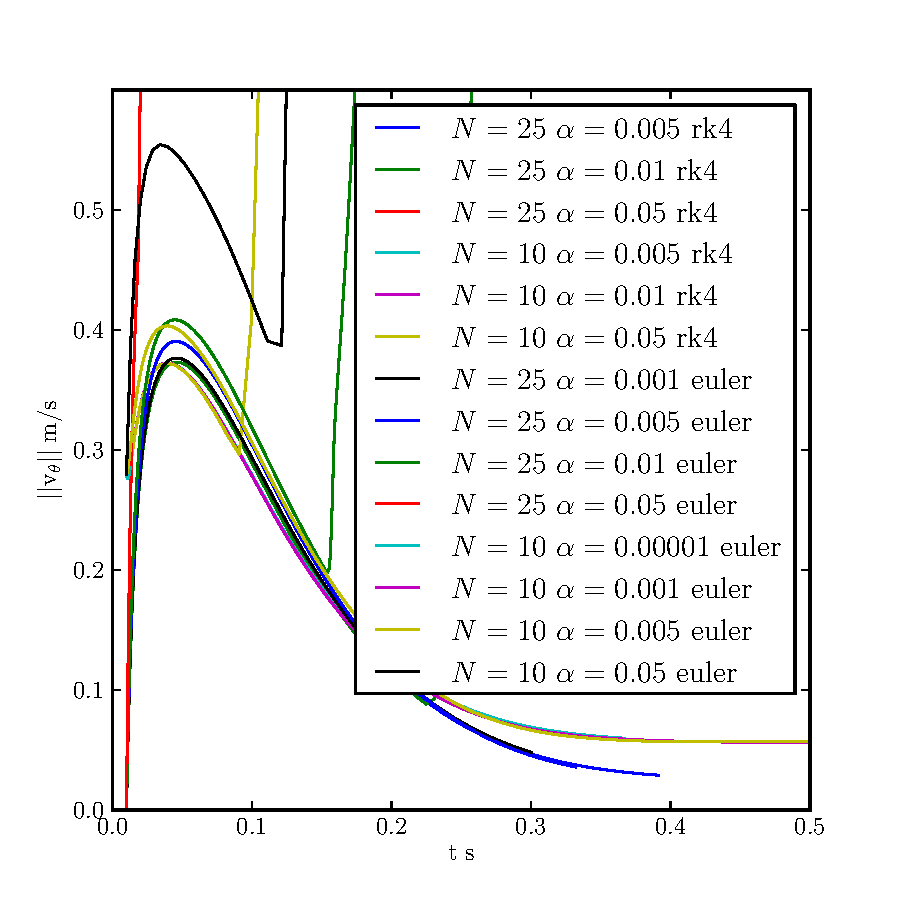
\includegraphics{fixed/normtheta.pdf}
\end{center}
\caption{Error norm for angular component.
}
\label{fix:normtheta}
\end{figure}

\begin{figure}
\begin{center}
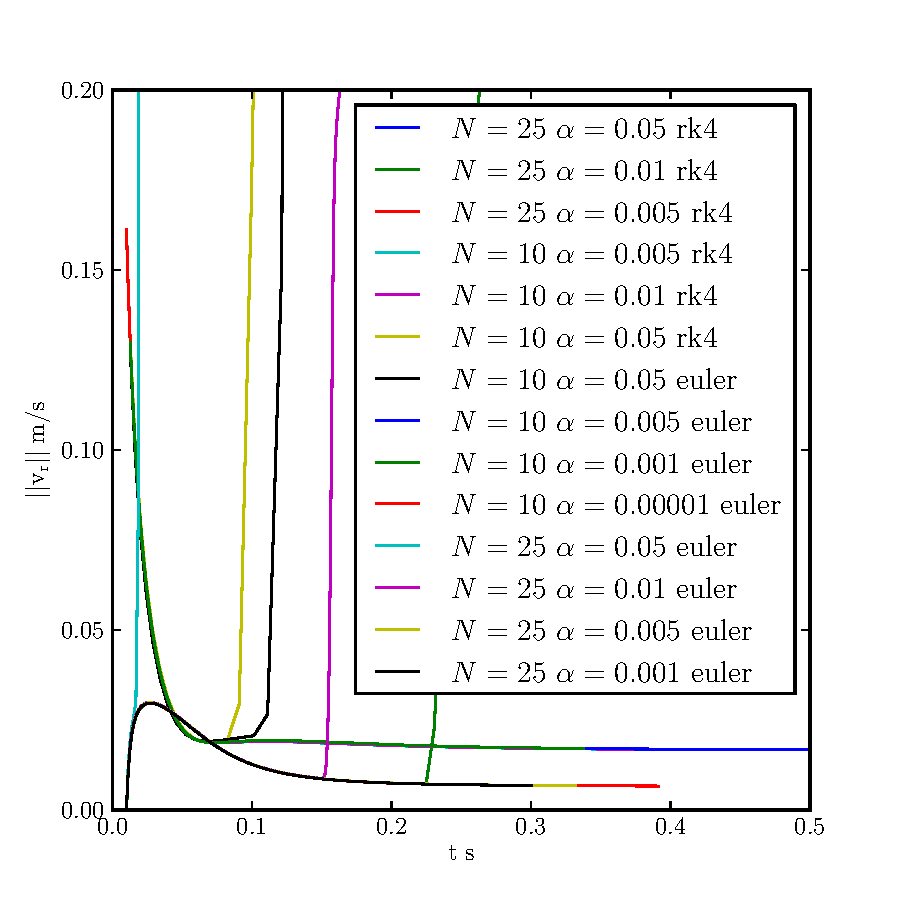
\includegraphics{fixed/normr.pdf}
\end{center}
\caption{Error norm for radial component.
}
\label{fix:normr}
\end{figure}


